Rozdział \ref{subsec:dwuwymiarowe_kopuly_probal} pokazał, że kopuły można intuicyjnie rozumieć jako modele zależności. W tej sekcji spojrzymy na nie z dualnej perspektywy, jako na dystrybuanty, co pozwoli nam zdefiniować użyteczne narzędzia do analizy charakteru tej zależności.

\begin{df}[Gęstość kopuły]
	Niech $C$ będzie $d$-wymiarową (jednostajnie ciągłą) kopułą. Gęstością tej kopuły nazywamy funkcję
	\begin{equation}
		c(u_1, \dots, u_d) = \frac{\partial^d}{\partial u_1\dots \partial u_d}C(u_1, \dots, u_d).
		\label{eq:copula_density}
	\end{equation}
\end{df}


Widzimy, że równanie \ref{eq:copula_density} jest jedynie przeniesieniem terminu gęstości wielowymiarowego rozkładu na grunt kopuł. Zanim zaczniemy wizualizować gęstości konkretnych kopuł, warto wspomnieć, że Sklar w \cite{Sklar_Theorem} podaje również alternatywną wersję swojego twierdzenia o istnieniu kopuły, tym razem w języku gęstości. Sens i zastosowania twierdzenia pozostają takie same jak dla twierdzenia \ref{thm:sklar_theorem}.
\begin{thm}[Twierdzenie Sklara: gęstość kopuły]
	Niech $X$ będzie $d$-wymiarowym wektorem losowym o dystrybuancie rozkładu łącznego $F$, oraz rozkładami brzegowymi $F_i$, $i=1, \dots, d$. Wtedy rozkład łączny może być wyrażony jako		$$F(x_1, \dots, x_d) = C(F_1(x_1), \dots, F_d(x_d)),$$
	lub równoważnie w terminach gęstości poprzez:
	$$ f(x_1, \dots, x_d) = c(F_1(x_1), \dots, F_d(x_d))\cdot f_1(x_1)\dots f_d(x_d),$$
	dla pewnej $d$-wymiarowej kopuli $C$, o gęstości $c$. Dla rozkładów bezwzględnie ciągłych, kopuła $C$ jest jednoznacznie określona.\\
	Zachodzi również twierdzenie odwrotne: kopuła związana z wielowymiarowym rozkładem $F$ o rozkładach brzegowych $F_1, \dots F_d$ może być wyrażona jako:
	$$C(u_1, \dots, u_d) = F(F_1^{-1}(u_1), \dots, F_d^{-1}(u_d)),$$
	a jej gęstość wyraża się poprzez:
	$$c(u_1, \dots, u_d) = \frac{f(F_1^{-1}(u_1), \dots, F_d^{-1}(u_d))}{f_1(F_1^{-1}(u_1))\dots f_d(F_d^{-1}(u_d))}$$
	\label{thm:sklar_theorem_density}
\end{thm}

Resztę rozdziału stanowić będzie omówienie różnych rodzin kopuł o istotnych zastosowaniach w praktyce. Będziemy prezentować ich gęstości, ponieważ w intuicyjny sposób przedstawiają one mapę osłabień i nasileń współzależności dla konkretnych kopuł. Informatywne w tym względzie są ich wykresy konturowe, przedstawiające izohipsy powierzchni gęstości. Standardowo przedstawia się je w naturalnej \emph{skali kopuły}, tzn. na kwadracie jednostkowym wizualizuje się bezpośrednio gęstość kopuły:
$$ c(u, v)\text{, dla } (u, v) \in [0, 1]^2.$$
Pomocna jest jednak również wizualizacja w \emph{skali brzegowo-znormalizowanej}, czyli po dokonaniu transformacji przez dystrybuantę $\Phi$ i gęstość $\phi$ standardowego rozkładu normalnego:
 $$ g(x, y) = c(\Phi(x), \Phi(y))\phi(x)\phi(y)\textit{, dla }(x,y)\in\R^2.$$
Powyższa transformacja nie wizualizuje już gęstości kopuły $c$, ale raczej gęstość rozkładu wielowymiarowego $g$, który powstałby gdybyśmy kopułą $c$ połączyli zmienne ze standardowego rozkładu normalnego, zgodnie z twierdzeniem \ref{thm:sklar_theorem}. Ta reprezentacja jest bardzo intuicyjna, ponieważ podstawowe kursy statystyki przyzwyczajają ludzkie oko do utożsamiania silnej/słabej korelacji z wydłużonymi/okrągłymi elipsami tworzonymi przez gęstość wielowymiarowego rozkładu normalnego. Reprezentacja w skali brzegowo-znormalizowanej jest intuicyjna, ponieważ dla kopuły gaussowskiej pokazuje dokładnie te same, znane elipsy. Natomiast w przypadku innych kopuł, obserwujemy rozbieżność izohips od eliptycznego kształtu co daje się łatwo zinterpretować. 

W praktyce istnieją trzy główne nurty tworzenia kopuł. Można wykorzystać do tego twierdzenie Sklara \ref{thm:sklar_theorem} jako twierdzenie konstrukcyjne, tj. wziąć pewien istniejący, znany rozkład wielowymiarowy, zaaplikować \emph{PIT} (\ref{def:PIT}) do jego rozkładów brzegowych i odzyskać w ten sposób $C$ z twierdzenia Sklara. Drugą metodą konstrukcji kopuł jest zdefiniowanie ich przez tzw. \emph{generator} - powstają w ten sposób kopuły archimedejskie. Trzeci sposób natomiast to rozszerzenie \emph{extreme-value theory} z jedego do wielu wymiarów, co skutkuje powstaniem kopuł typu \emph{extreme-value}.\\

\subsubsection{Rodzina kopuł eliptycznych}

Kopuły eliptyczne są przykładem konstrukcji kopuł poprzez bezpośrednią aplikację twierdzenia Sklara \ref{thm:sklar_theorem} do rozkładów eliptycznych, zdefiniowanych na początku rozdziału \ref{sec:rozklady_wielowymiarowe}. Można więc tę konstrukcję rozumieć jako implikowanie struktury zależności z wielowymiarowych rozkładów, poprzez wyeliminowanie wpływu rozkładów brzegowych. W tej rodzinie zobaczymy przede wszystkim kopuły reprezentujące zależności ,,implikowane" z wielowymiarowego rozkładu normalnego, czy wielowymiarowego rozkładu $t$.

\begin{df}[Kopuła produktowa]
	Kopuła produktowa to kopuła o gęstości:
	
	$$ c(u_1, u_2) = 1.$$
	
\end{df}
\begin{figure}[h]
	\centering
	\begin{minipage}{0.5\linewidth}
		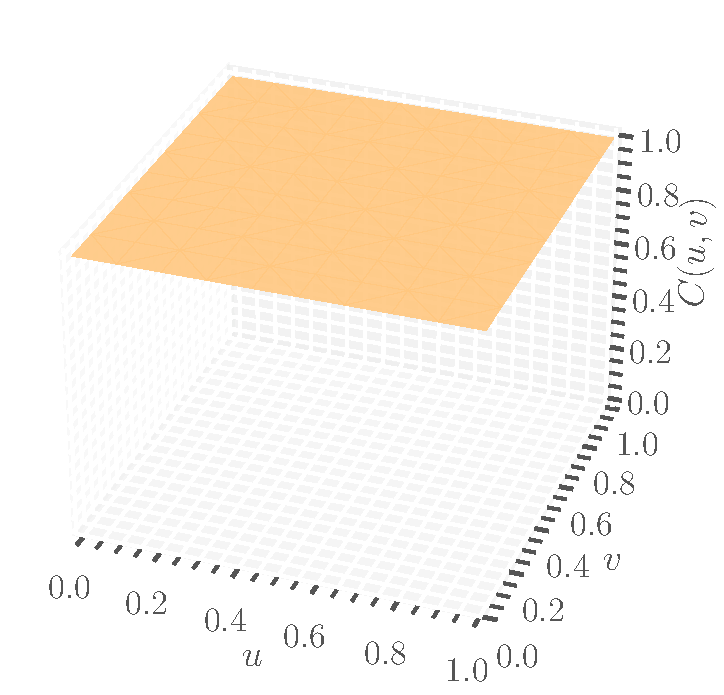
\includegraphics[width=\linewidth]{02_IndependenceCopula_density}
	\end{minipage}
	\begin{minipage}{0.45\linewidth}
		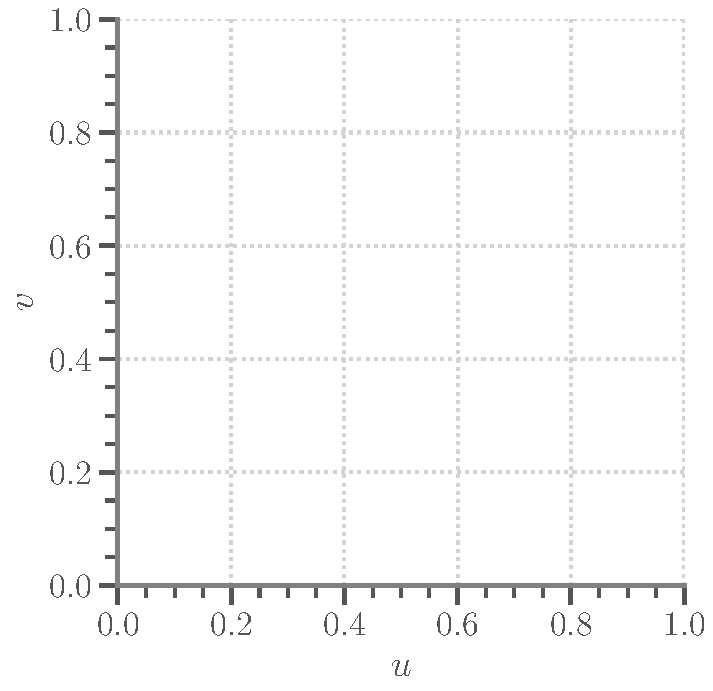
\includegraphics[width=.8\linewidth]{02_IndependenceCopula_contour}
		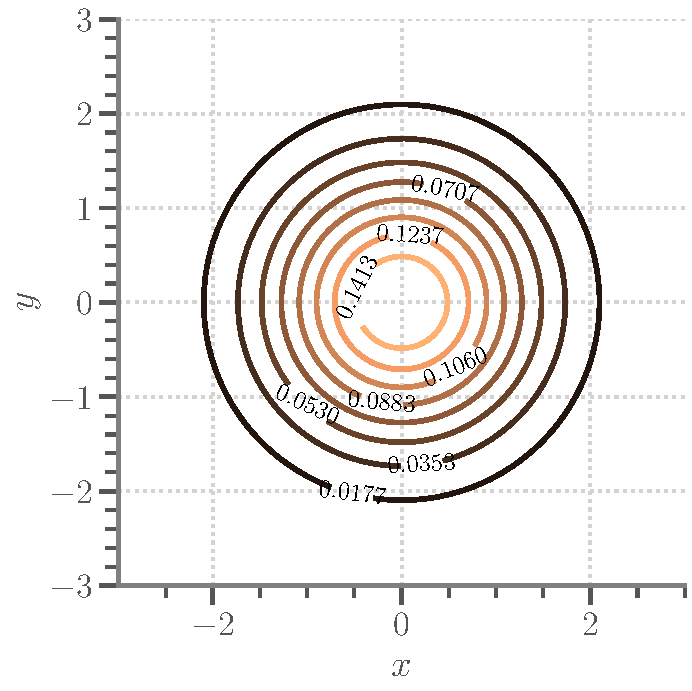
\includegraphics[width=.8\linewidth]{02_IndependenceCopula_contour_norm}
	\end{minipage}
	\caption{\textbf{Kopuła produktowa.} Powierzchnia gęstości (lewy panel), jej kontur w skali kopuły (prawy górny panel) i kontur w skali brzegowo-znormalizowanej (prawy dolny panel). \label{fig:product_copula_density}}
\end{figure}

Dystrybuantę tej kopuły przedstawiliśmy wcześniej na rysunku \ref{fig:prod_copula}, jednak w tym rozdziale pokazujemy ją w nieco innym świetle. Jednakowa gęstość widoczna na rysunku \ref{fig:product_copula_density} w każdym punkcie kwadratu jednostkowego mówi, że każda para $(u, v) \in [0,1]^2$ ma jednakową szansę na występienie, więc nie ma żadnej zależności między $U$ a $V$. Jest to zgodne z uwagą z rozdziału \ref{subsec:dwuwymiarowe_kopuly_probal}, mówiącą że ta kopuła odpowiada niezależnemu połączeniu zmiennych losowych. Zwróćmy uwagę na prawy dolny panel rysunku \ref{fig:product_copula_density}, który prezentuje izohipsy w skali brzegowo-znormalizowanej. Widzimy koncentryczne okręgi, kojarzące się z wielowymiarowym rozkładem normalnym o korelacji $0$. Istotnie, kopuła produktowa reprezentuje strukturę zależności w tym wielowymiarowym rozkładzie.

\begin{df}[Kopuła gaussowska]
	Kopuła gaussowska o korelacji $\rho$, to kopuła zadana wzorem:
	
	$$ C(u_1, u_2; \rho) = \Phi_2(\Phi^{-1}(u_1), \Phi^{-1}(u_2);\rho),$$
	
	gdzie $\Phi$ oraz $\phi$ to odpowiednio dystrybuanta i gęstość standardowego rozkładu normalnego. Gęstość kopuły gaussowskiej zadana jest wzorem:
	$$ c(u_1, u_2; \rho) = \frac{1}{\phi(x_1)\phi(x_2)} \frac{1}{\sqrt{1-\rho^2}}\exp\bigg[-\frac{\rho^2(x_1^2+x_2^2) - 2\rho x_1 x_2}{2(1-\rho^2)}\bigg],$$
	gdzie $x_i\coloneqq \Phi^{-1}(u_i)$.
\end{df}
\begin{figure}[h]
	\centering
	\begin{minipage}{0.5\linewidth}
		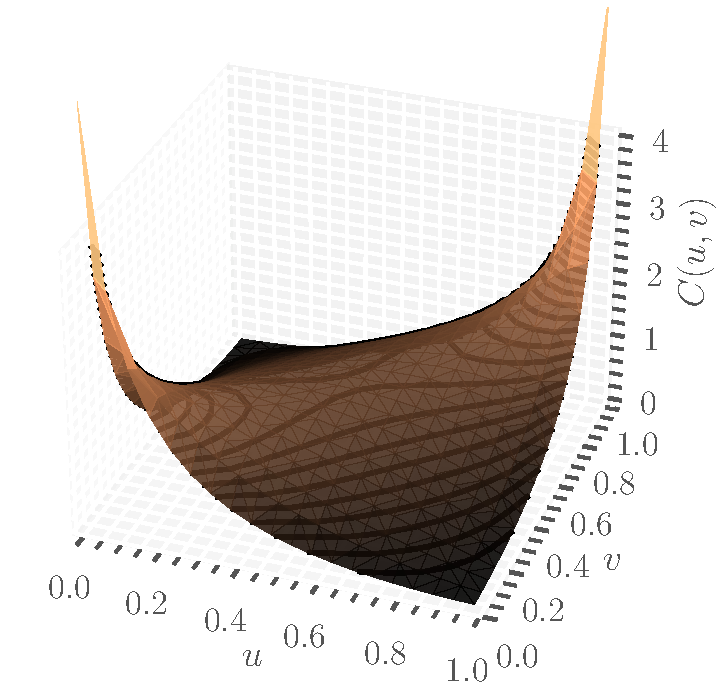
\includegraphics[width=\linewidth]{02_GaussianCopula_density}
	\end{minipage}
	\begin{minipage}{0.45\linewidth}
		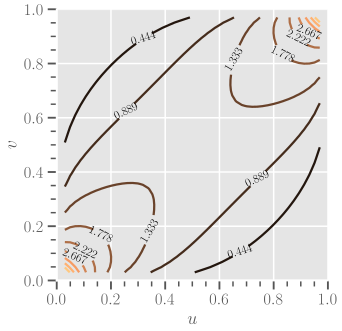
\includegraphics[width=.8\linewidth]{02_GaussianCopula_contour}
		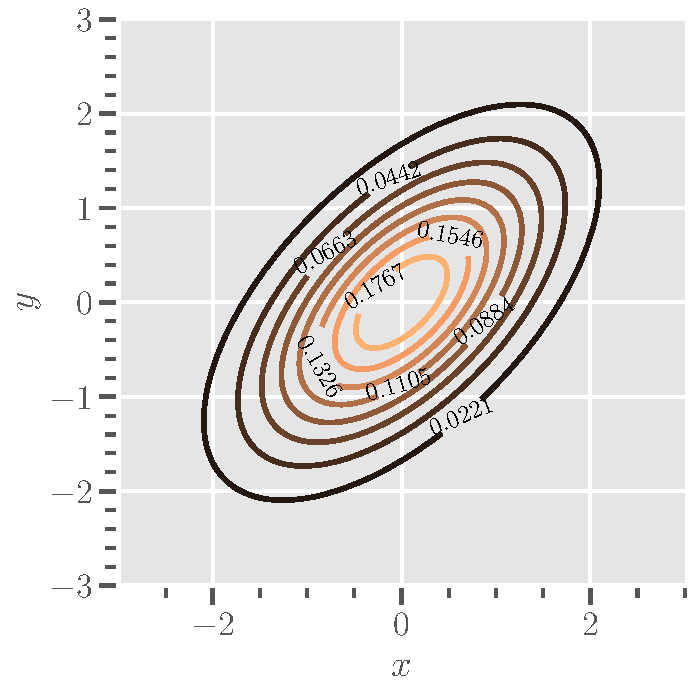
\includegraphics[width=.8\linewidth]{02_GaussianCopula_contour_norm}
	\end{minipage}
	\caption{\textbf{Kopuła gaussowska}, $\rho=0.6$, Powierzchnia gęstości (lewy panel), jej kontur w skali kopuły (prawy górny panel) i kontur w skali brzegowo-znormalizowanej (prawy dolny panel). \label{fig:gaussian_copula_density}}
\end{figure}

Kopuła gaussowska modeluje strukturę zależności implikowaną przez wielowymiarowy rozkład normalny, tj. wielowymiarowy rozkład normalny jest równoważny modelowi o normalnych rozkładach brzegowych, połączonych kopułą gaussowską. Rodzina kopuł gaussowskich jest wyczerpująca. Przykładowa powierzchnia gęstości oraz kontury kopuły gaussowskiej przedstawione są na rysunku \ref{fig:gaussian_copula_density}.

\begin{df}[Kopuła studenta]
	Kopuła studenta to jednoparametryczna kopuła o $\nu$ stopniach swobody i korelacji $\rho$ zadana jest gęstością:
	
	$$ C(u_1, u_2;\nu,\rho) = \frac{t(T_{\nu}^{-1}(v_1), T_{\nu}^{-1}(v_2);\nu,\rho)}{t_{\nu}(T_{\nu}^{-1}(v_1))t_{\nu}(T_{\nu}^{-1}(v_2))}.$$
\end{df}
\begin{figure}[h]
	\centering
	\begin{minipage}{0.5\linewidth}
		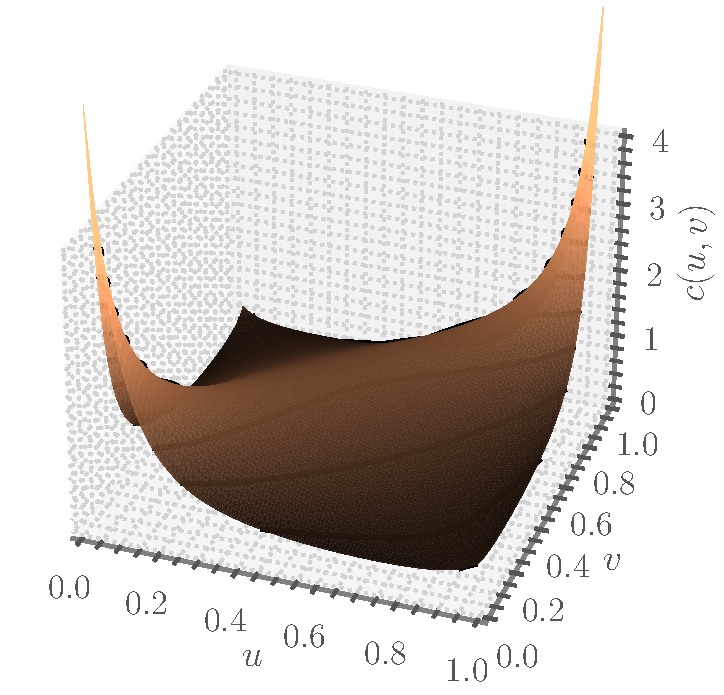
\includegraphics[width=\linewidth]{02_StudentCopula_density}
	\end{minipage}
	\begin{minipage}{0.45\linewidth}
		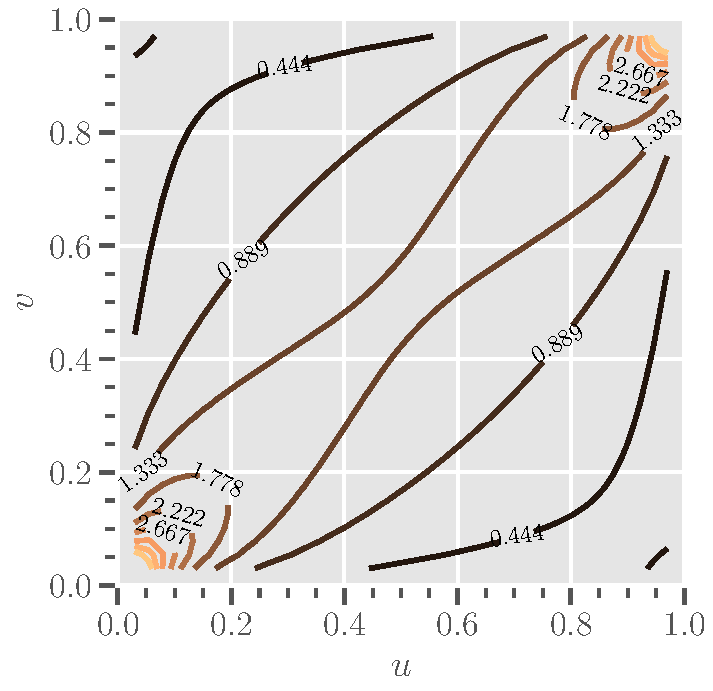
\includegraphics[width=.8\linewidth]{02_StudentCopula_contour}
		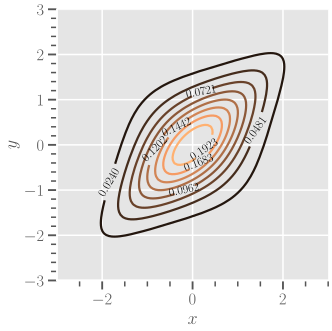
\includegraphics[width=.8\linewidth]{02_StudentCopula_contour_norm}
	\end{minipage}
	\caption{\textbf{Kopuła studenta}, $\nu=3, \rho=0.5$: powierzchnia gęstości (lewy panel), jej kontur w skali kopuły (prawy górny panel) i kontur w skali brzegowo-znormalizowanej (prawy dolny panel). \label{fig:student_copula_density}}
\end{figure}
Kopuła studenta, podobnie do gaussowskiej, jest implikowana z rozkładu eliptycznego studenta. Oznacza to, że wielowymiarowy rozkład studenta jest równoważny modelowi o rozkładach brzegowych $t$ połączonych kopułą studenta. Wraz z rosnącą ilością stopni swobody kopuła studenta zbiega do gaussowskiej. Ta rodzina nie jest jednak wyczerpująca, ponieważ nawet przy $\rho=0$, dla żadnej skończonej liczby stopni swobody nie zawiera w sobie $C^{\perp}$.\\

Kopuły eliptyczne cieszą się dużą popularnością w instytucjach finansowych, ponieważ mają swoje naturalne $d$-wymiarowe rozszerzenia. Kopuły uważane są mimo wszystko za skomplikowane modele, i w obliczu szczegółowych regulacji nakładanych na wewnętrzne modele (np. w podejściu AMA do modelowania ryzyka operacyjnego \cite{BaselII}) dużo łatwiej jest uzasadnić i utrzymać w produkcji model bazujący na kilku intuicyjnych parametrach. Z tego powodu, kopuła $t$ studenta jest najczęściej wybieraną w praktyce - pozwala bowiem na modelowanie ciężkich ogonów i korelacji, a jednocześnie jest zaledwie dwuparametryczna (\cite{OpRisk}).\\

\subsubsection{Rodzina kopuł archimedejskich}

\begin{df}[Kopuły archimedejskie]
		Niech $\mathcal{F}$ będzie zbiorem ciągłych, jednostajnie malejących i wypukłych funkcji $\phi \colon [0,1] \mapsto [0, \infty]$, takich, że $\phi(1) = 0$. Wtedy
		
		$$ C(u_1, u_2) = \phi^{[-1]}(\phi(u_1)+\phi(u_2))$$
		jest kopułą. Uściślając, nazwiemy ją kopułą archimedejską o generatorze $\phi$. W powyższej definicji, przez $\phi^{[-1]}$ rozumiemy pseudoodwrotność $\phi$, czyli funkcję $\phi^{[-1]}\colon [0, \infty] \mapsto [0, 1]$ zadaną przez:
		
		$$ \phi^{[-1]}(t) \coloneqq \phi^{-1}(t) \1_{\{0\leqslant t \leqslant \phi(0)\}}. $$
\end{df}

Ta rodzina została wprowadzona została przez Claytona w \cite{Clayton1972} w kontekście modelowania zapadalności na choroby przewlekłe, gdzie posłużyła do opisania zależności w aktuarialnych tabelach średniego dalszego trwania życia. Dziś kopuły archimedejskie wymieniane są pośród najczęściej wykorzystywanych do analizy zależności dwuwymiarowych. W przeciwieńswie do rodziny eliptycznej, kopuły z rodziny archimedejskiej potrafią modelować asymetryczne zależności. Oznacza to, że osiągalne są w nich struktury, w których dolne ogony zmiennych losowych są bardziej od siebie zależne niż ogony prawe i \emph{vice versa}. Najprostsze tego zastosowanie to model zwrotów na rynku akcji, które przejawiają silniejszą korelację w lewym ogonie niż w prawym (\cite{AssymetricEquityDependency}). \\
Ponadto, kopuły archimedejskie pozwalają wyrazić $\tau$ Kendalla, czy współczynnik zależności ogonów w języku generatora, co powoduje, że są łatwe w estymacji.

\begin{prop}
	Dla dwóch zmiennych losowych połączonych kopułą archimedejską o generatorze $\phi$, współczynnik $\tau$ Kendalla ma reprezentację:
	
	$$ \tau = 4\int_{[0, 1]}\frac{\phi(v)}{\phi'(v)}dv + 1.$$
	
	Współczynniki zależności ogonów wyrażają się natomiast przez:
	
	\begin{equation}
		\begin{split}
		\lambda^{l}&=2\lim\limits_{s\to\infty}\frac{\phi'(s)}{\phi(2s)} \\
		\lambda^{u}&=2-2\lim\limits_{s\to0^{+}}\frac{\phi'(s)}{\phi(2s)}
		\end{split}
	\end{equation}
\end{prop}
Powyższe uwagi powoduja, że rodzina kopuł archimedejskich jest zazwyczaj wystarczająco dobra dla większości praktycznych zastosowań. Do tej klasy należą m.in kopuły Claytona, Gumbela czy Franka.

\begin{df}[Kopuła Claytona]
	Kopuła Claytona to kopuła archimedejska o generatorze $\phi(t;\delta) = \frac{1}{\delta}(t^{-\delta}-1)$. Jest ona jednoparametryczną kopułą, wyrażoną poprzez dystrybuantę zadaną wzorem:
	
	$$ C(u_1, u_2; \delta) = (u_1 ^{-\delta} + u_2^{-\delta} - 1)^{-\frac{1}{\delta}},$$
	dla $\delta \in [-1, 0) \cup (0, \infty).$
\end{df}
\begin{prop}
	Dla kopuły Claytona o parametrze $\delta$, współczynnik Kendalla wynosi:
	$$ \tau = 1 - \frac{1}{\delta}.$$
	
	Współczynniki zależności ogonów wynoszą zaś odpowiednio:
	\begin{equation}
		\begin{split}
			\lambda^{l}&=2^{-\frac{1}{\delta}} \\
			\lambda^{u}&=0.
		\end{split}
	\end{equation}
\end{prop}
Kopuła Claytona pozwala modelować niesymetryczne zależności zmiennych losowych. Jest rodziną wyczerpującą, mamy bowiem: $C(u,v;\delta = 1) = C^{\perp}$, $C(u,v;\delta = -1) = C^{-}$, oraz $C(u,v;\delta \to \infty) \to C^{+}$. Rysunek \ref{fig:clayton_copula_density} przedstawia powierzchnię gęstości i kontury w przypadku $\delta = 1.2$. Na rysunku widoczny jest dobrze wpływ istnienia dolnego współczynnika zależności ogonów na kształt konturów i gęstości.

\begin{figure}[h]
	\centering
	\begin{minipage}{0.5\linewidth}
		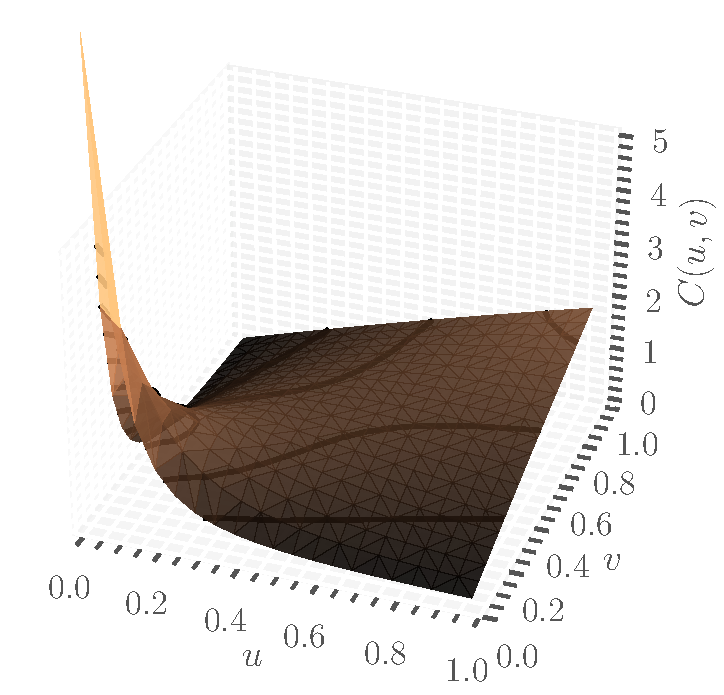
\includegraphics[width=\linewidth]{02_ClaytonCopula_density}
	\end{minipage}
	\begin{minipage}{0.45\linewidth}
		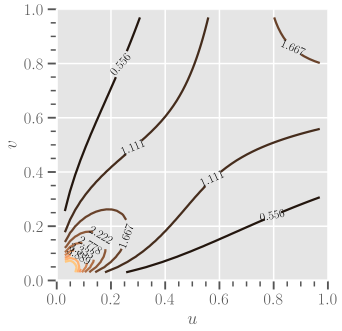
\includegraphics[width=.8\linewidth]{02_ClaytonCopula_contour}
		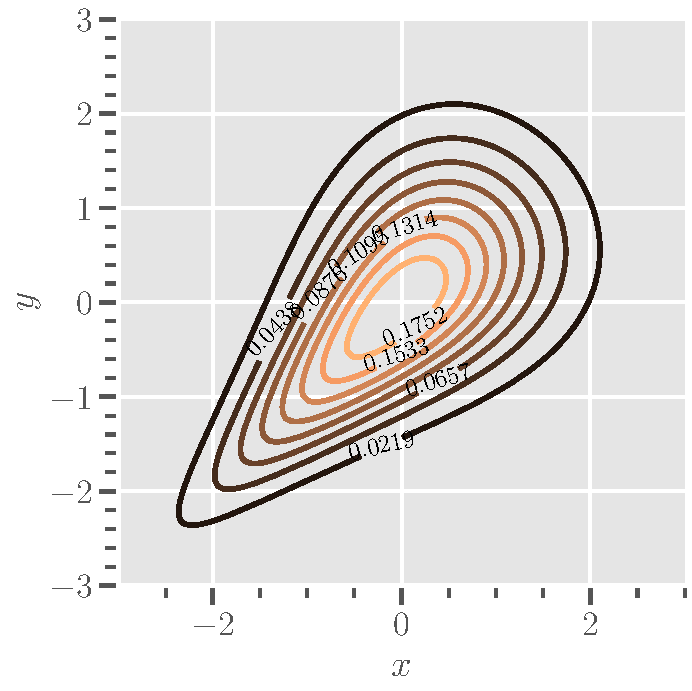
\includegraphics[width=.8\linewidth]{02_ClaytonCopula_contour_norm}
	\end{minipage}
	\caption{\textbf{Kopuła Claytona}, $\delta = 1.2$: powierzchnia gęstości (lewy panel), jej kontur w skali kopuły (prawy górny panel) i kontur w skali brzegowo-znormalizowanej (prawy dolny panel). \label{fig:clayton_copula_density}}
\end{figure}

\begin{df}[Kopuła Gumbela]
	Kopuła Gumbela to kopuła archimedejska o generatorze $\phi(t;\delta) = (-\ln t)^{\delta}$. Jest ona jednoparametryczną kopuła, wyrażoną poprzez dystrybuantę zadaną wzorem:
	
	$$ C(u_1, u_2; \delta) = \exp\big[-[(-\ln u_1)^\delta+(-\ln u_2)^\delta]^{\frac{1}{\delta}}\big],$$
	dla $\delta \geqslant 1.$
\end{df}
\begin{prop}
	Dla kopuły Gumbela o parametrze $\delta$, współczynnik Kendalla wynosi:
	$$ \tau = \frac{\delta}{\delta + 2}.$$
	
	Współczynniki zależności ogonów wynoszą zaś odpowiednio:
	\begin{equation}
		\begin{split}
			\lambda^{l}&=0\\
			\lambda^{u}&=2 - 2^{\frac{1}{\delta}}.
		\end{split}
	\end{equation}
\end{prop}
Kopuła Gumbela również pozwala modelować niesymetryczne zależności zmiennych losowych.  Rysunek \ref{fig:gumbel_copula_density} przedstawia powierzchnię gęstości i kontury w przypadku $\delta = 1.8$, gdzie widzimy powyższą niesymetryczność. Ta rodzina nie jest jednak wyczerpującą, ponieważ mamy jedynie $C(u,v;\delta = 1) = C^{\perp}$, oraz $C(u,v;\delta \to \infty) \to C^{+}$, natomiast kopuła $C^{-}$ nie jest częścią tej rodziny. \\
Kopuły Gumbela mogą więc posługiwać do modelowania jedynie dodatnich zależności, lub w granicznym przypadku niezależności. Nie przeszkodziło to jednak w skutecznej aplikacji tych kopuł do badań klinicznych, gdzie spopularyzował je Hougaard, w \cite{Hougaard1986} wykorzystując do testowania hipotez o pozytywnym wpływie leku przeciw guzom na długość życia szczurów w grupie leczenia.

\begin{figure}[h]
	\centering
	\begin{minipage}{0.5\linewidth}
		\includegraphics[width=\linewidth]{02_GumbelCopula_density}
	\end{minipage}
	\begin{minipage}{0.45\linewidth}
		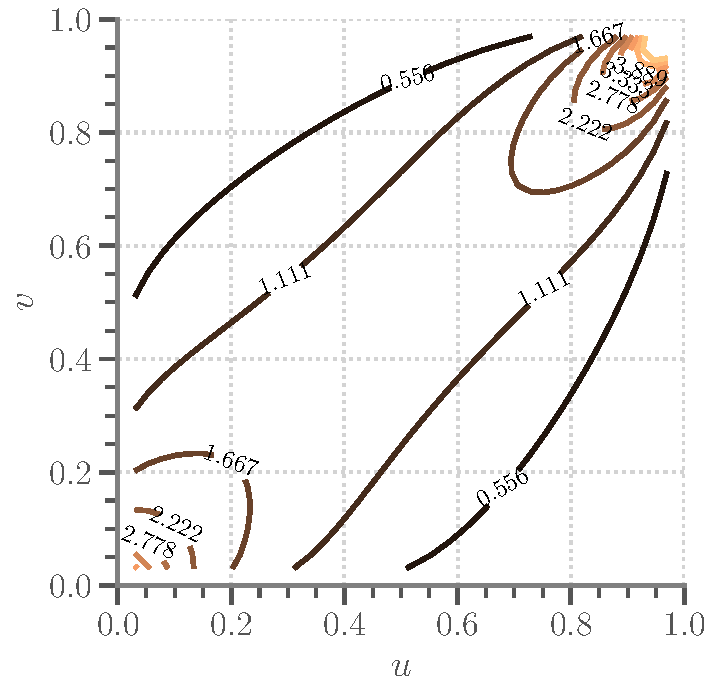
\includegraphics[width=.8\linewidth]{02_GumbelCopula_contour}
		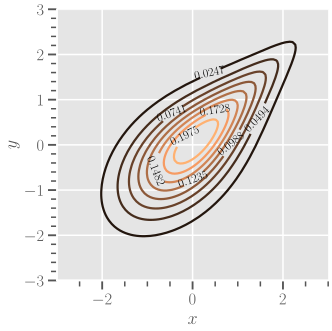
\includegraphics[width=.8\linewidth]{02_GumbelCopula_contour_norm}
	\end{minipage}
	\caption{\textbf{Kopuła Gumbela}, $\delta = 1.8$: powierzchnia gęstości (lewy panel), jej kontur w skali kopuły (prawy górny panel) i kontur w skali brzegowo-znormalizowanej (prawy dolny panel). \label{fig:gumbel_copula_density}}
\end{figure}

\begin{df}[Kopuła Franka]
	Kopuła Franka to kopuła archimedejska o generatorze $\phi(t;\delta) = -\ln\frac{\exp(-\alpha t) - 1}{\exp(-\alpha)-1}$. Jest ona jednoparametryczną kopuła, wyrażoną poprzez dystrybuantę zadaną wzorem:
	
	$$ C(u_1, u_2; \delta) = -\frac{1}{\delta}\ln\bigg[ \frac{1}{1-e^{-\delta}}\big[(1-e^{-\delta}) - (1-e^{-\delta u_1})(1-e^{-\delta u_2})\big] \bigg],$$
	dla $\delta \in (-\infty; 0) \cup (0; \infty).$
\end{df}
\begin{prop}
	Dla kopuły Franka o parametrze $\delta$, współczynnik Kendalla wynosi:
	$$ \tau = 1 + 4[D(\delta) - 1]/\delta,$$
	gdzie $D(\alpha)$ to:
	$$ D(\alpha) = \frac{1}{\alpha} \int_{0}^{\alpha} \frac{t}{\exp(t) - 1}dt.$$
		
	Współczynniki zależności ogonów wynoszą zaś odpowiednio:
	\begin{equation}
		\begin{split}
			\lambda^{l}&=0\\
			\lambda^{u}&=0.
		\end{split}
	\end{equation}
\end{prop}

\begin{figure}[h]
	\centering
	\begin{minipage}{0.5\linewidth}
		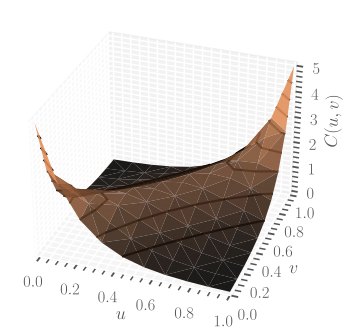
\includegraphics[width=\linewidth]{02_FrankCopula_density}
	\end{minipage}
	\begin{minipage}{0.45\linewidth}
		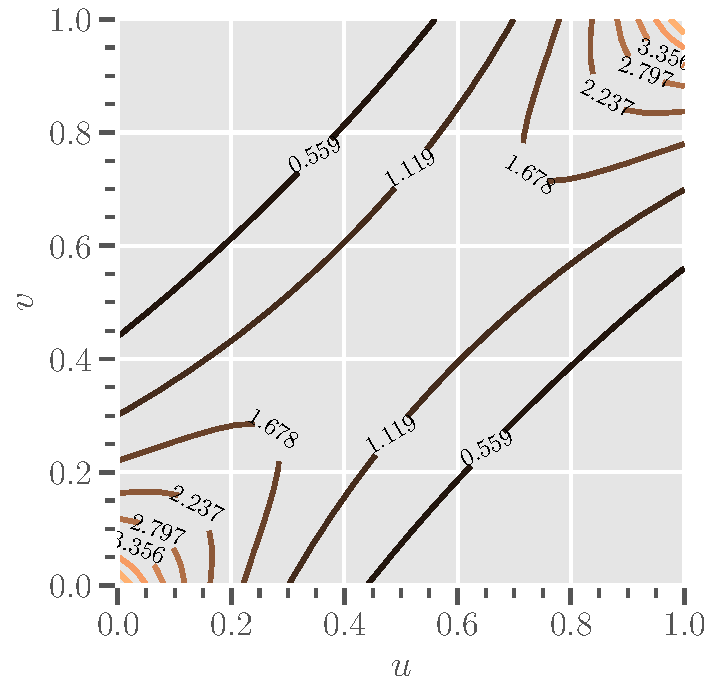
\includegraphics[width=.8\linewidth]{02_FrankCopula_contour}
		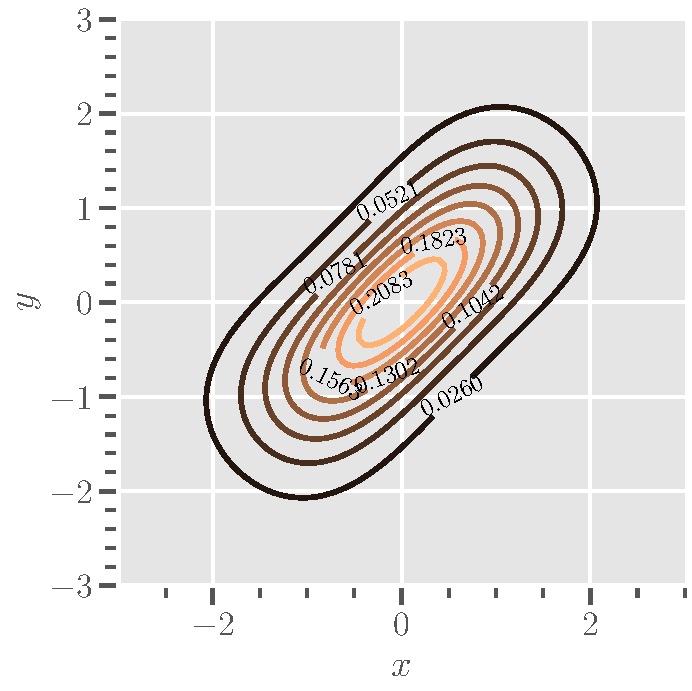
\includegraphics[width=.8\linewidth]{02_FrankCopula_contour_norm}
	\end{minipage}
	\caption{\textbf{Kopuła Franka}, $\delta = 5$: powierzchnia gęstości (lewy panel), jej kontur w skali kopuły (prawy górny panel) i kontur w skali brzegowo-znormalizowanej (prawy dolny panel). \label{fig:frank_copula_density}}
\end{figure}

Rodzina kopuł Franka jest rodziną wyczerpującą, bowiem $C(u,v;\delta = 0) = C^{\perp}$, $C(u,v;\delta \to \infty) \to C^{+}$, oraz $C(u,v;\delta \to -\infty) \to C^{-}$ . Kopuła Franka jako jedyna z wymienionych kopuł archimedejskich jest symetryczna. Rysunek \ref{fig:frank_copula_density} przedstawia powierzchnię gęstości i kontury w przypadku $\delta = 5$. \\
Jedno z ciekawych jej zastosowań, przedstawia \cite{Jianwei2021}. W swojej pracy Jianwei rozważa problem optymalizacji częstości ładowania pojazdów elektrycznych. Kopuła Franka jest przez niego używana do modelowania zależności między siłą wiatru, a ilością energii z ogniw fotowoltaicznych, co wykorzystuje do wyznaczenia optymalnej strategii ładowania pojazdu, która stabilizuje popyt/podaż na energię w sieci energetycznej, skutkując niższymi kosztami utrzymania pojazdu. 

\subsubsection{Rodzina kopuł \emph{extreme-value}}

Ostatnią z prezentowanych metod konstrukcji kopuł jest konstrukcja asymptotyczna, poprzez teorię wartości ekstremalnych.\\
Zakładając, że $X_1$ i $X_2$ są dwoma zmiennymi losowymi o rozkładach $F_1$, $F_2$, zdefiniujemy kopułę \emph{extreme-value} jako kopułę odpowiadającą za zależność pomiędzy maksimum z $n$ realizacji $X_1$ a maksimum z $n$ realizacji $X_2$. 

\begin{df}[Kopuła \emph{extreme-value}]
	Dwuwymiarowa kopuła $C$ nazywana jest kopułą \emph{extreme-value}, jeżeli istnieje dwuwymiarowa kopuła $C_X$, taka że dla $n\to\infty$ mamy:
	
	$$ [C_X(u_1^{\frac{1}{n}}, u_2^{\frac{1}{n}})]^n \to C(u_1, u_2) \forall_{(u_1, u_2)}\in [0,1]^2.$$
	
	Mówimy wówczas, że kopuła $C_X$ jest w obszarze przyciągania kopuły $C$.
\end{df}

To samo można zdefiniować posługując się pojęciem kopuł \emph{max-stabilnych}
\begin{df}[Kopuła max-stabilna]
	Dwuwymiarowa kopuła $C$ nazywana jest kopułą max-stabilną, jeśli spełnia warunek:
	
	$$ C(u_1, u_2) = [C(u_1^{\frac{1}{n}}, u_2^{\frac{1}{n}})]^n,$$
	Dla każdej liczby całkowitej $n\geqslant 1$, oraz dla każdej pary ${(u_1, u_2)}\in [0,1]^2.$
	
\end{df}
\begin{thm}
	Dwuwymiarowa kopuła $C$ jest kopułą \emph{extreme-value}, tylko i tylko wtedy gdy jest max-stabilna.
\end{thm}

Przykładem kopuły \emph{extreme-value} z podanych już wcześniej jest kopuła Gumbela. Inną, nietypową, ale często spotykaną kopułą z tej rodziny jest kopuła Marshalla-Olkina.

\begin{df}[Kopuła Marshalla-Olkina]
	Dwuwymiarową kopułą Marshalla-Olkina o parametrach $m$ i $n$ nazwiemy kopułę o dystrybuancie:
	
	$$ C(u_1, u_2; m,n) = \min[u_1^{1-m}u_2; u_1u_2^{1-n}].$$
	Gęstość tej kopuły zadana jest przez:
	
	$$
	c(u_1, u_2;m,n)=
	\begin{cases}
		(1-m)u_1^{-m},\text{ dla }u_1^m>u_2^n\\
		(1-n)u_2^{-n},\text{ dla }u_1^m<u_2^n
	\end{cases}
	$$	
\end{df}
\begin{prop}
	Dla kopuły Marshalla-Olkina o parametrach $m,n$, współczynnik Kendalla wynosi:
	$$ \tau = \frac{mn}{m-mn+n}.$$
	
	Współczynniki zależności ogonów wynoszą zaś odpowiednio:
	\begin{equation}
		\begin{split}
			\lambda^{l}&=0\\
			\lambda^{u}&=min(m,n).
		\end{split}
	\end{equation}
\end{prop}
Kopuła Marshalla-Olkina jest nietypowa, bo posiada część ciągłą, o powyższej gęstości, jak i część singularną wzdłuz krzywej $u_1^m=u_2^n$. Ta rodzina nie jest wyczerpująca, ponieważ nie zawiera $C^{-}$. Natomiast dla $m=0 \vee n=0$ mamy $C^{\perp}$, a przy $m=1=n$ dostajemy $C^{+}$. Wizualizację kopuli Marshalla-Olkina można zobaczyć na rysunku \ref{fig:marshall_olkin_copula_density}.\\
Kopuły Marshalla-Olkina powstają naturalnie w teorii niezawodności systemów. Rozważając system o wielu komponentach, gdzie awaria dowolnego komponentu powoduje awarię całego systemu, w klasycznym podejściu zakłada się rozkład wykładniczy dla czasu życia każdego z komponentów (z powodu braku pamięci), oraz niezależność między komponentami. W praktyce jednak, czasy do awarii poszczególnych komponentów nie są niezależne. Rozważenie momentu awarii systemu jako moment pierwszej awarii któregoś z jego komponentów prowadzi właśnie do kopuły Marshalla-Olkina \cite{Matus2019}.\\

\begin{figure}[h]
	\centering
	\begin{minipage}{0.5\linewidth}
		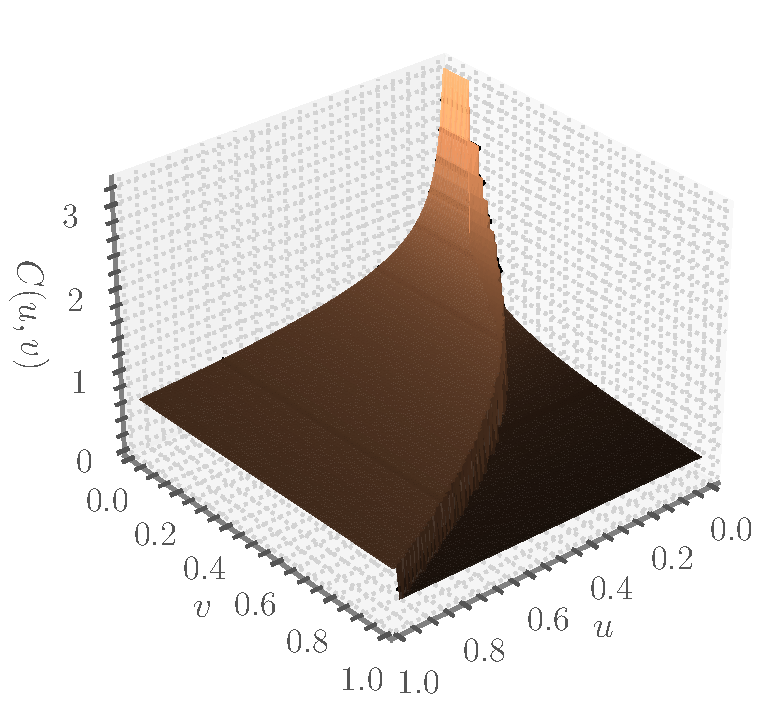
\includegraphics[width=\linewidth]{02_MarshallOlkinCopula_density}
	\end{minipage}
	\begin{minipage}{0.45\linewidth}
		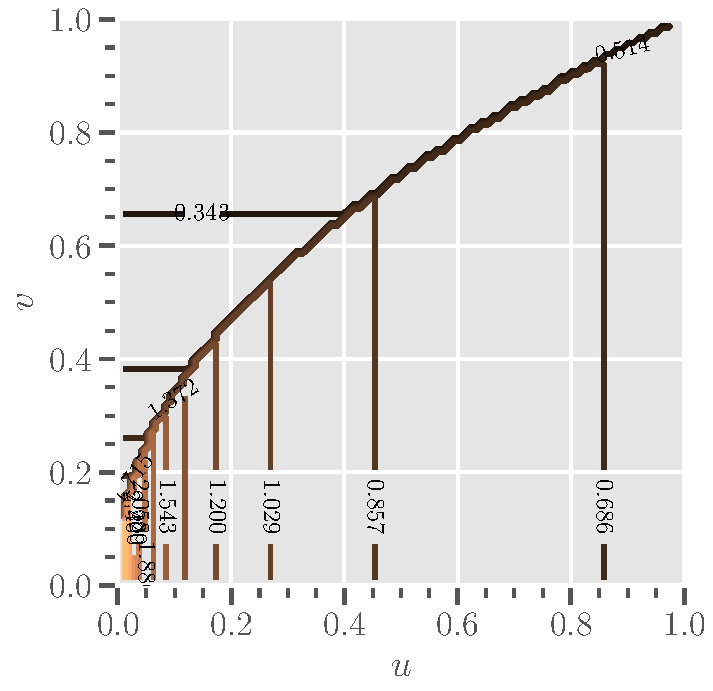
\includegraphics[width=.8\linewidth]{02_MarshallOlkinCopula_contour}
		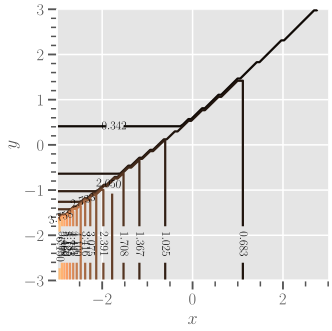
\includegraphics[width=.8\linewidth]{02_MarshallOlkinCopula_contour_norm}
	\end{minipage}
	\caption{\textbf{Kopuła Marshalla-Olkina}, $m=0.35,n=0.75$: powierzchnia gęstości (lewy panel), kontur w skali kopuły (prawy górny panel), kontur w skali brzegowo-znormalizowanej (prawy dolny panel). \label{fig:marshall_olkin_copula_density}}
\end{figure}



